Логическая (даталогическая) модель --- это схема базы данных на основе конкретной модели данных, набор схем отношений с указанием первичных ключей, а также «связей» между отношениями, представляющих собой внешние ключи.

Модель <<Сущность-связь>> (ER-модель) представлена на рисунке \ref{idef1x:idef1x}.

\begin{figure}[h!]
\center{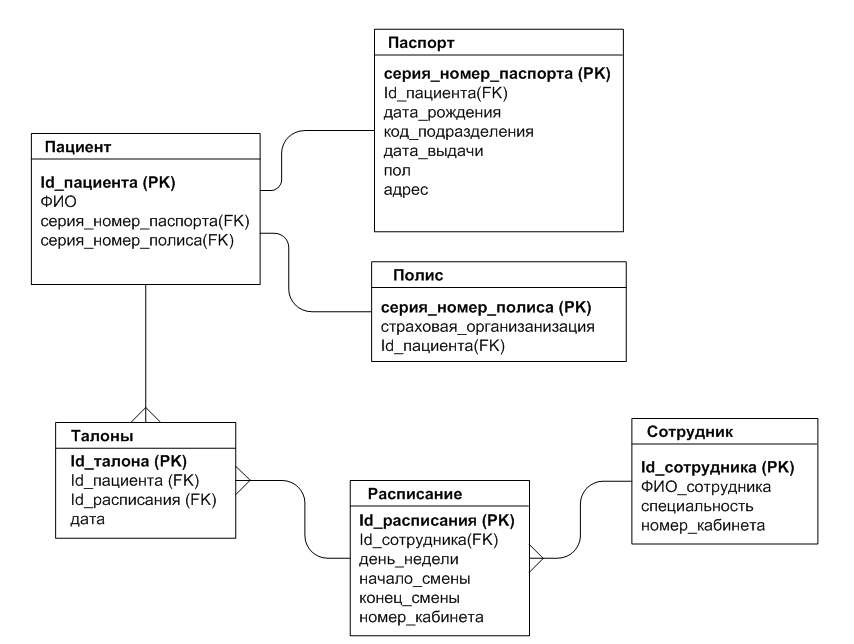
\includegraphics[width=0.9\linewidth]{idef1x}}
\caption{Диаграмма IDEF1X (модель <<Сущность-связь>>)}
\label{idef1x:idef1x}
\end{figure} 

\clearpage
